\documentclass[a4paper,12pt]{article}
\usepackage{amssymb}
\usepackage{amsmath}
\usepackage[utf8]{inputenc}
\usepackage[german]{babel}
\usepackage[T1]{fontenc}
\usepackage[margin=2.5cm]{geometry}
\usepackage{booktabs}
\usepackage{pdfpages}

\usepackage{hyperref}

\makeglossary 



\newcommand{\authorName}{Hendrik Lüth}
\newcommand{\Arbeitgeber}{Ausbildungswerkstatt der Marine}
\newcommand{\projekt}{DDS-Signalgenerator}
\title{\projekt}
\author{\authorName}

\begin{document}
 \pagenumbering{roman}
 \maketitle
 \setcounter{page}{2}
 \tableofcontents
 \clearpage
 \pagenumbering{arabic}
 
\section{Zielbestimmung}
Es soll ein Signalgenerator angefertigt werden. Hierbei ist sich an den Schalplan und die dort verzeichneten Werte zu halten.
Die verwendeten Bauteile sollen, soweit möglich, SMD-Bauteile sein.\\
Der Umfang des Auftrages umfasst:
\begin{itemize}
\item{das Layouten und Herstellen der Platine}
\item{Beschaffung der Bauteile}
\item{das Bestücken der Platine}
\item{das programmieren einer Software für den Mikrocontroller des Signalgenerators}
\end{itemize}

\section{Funktionale Anforderungen}

\subsection{Platine \& Layout}

Da ein bestimmtes Gehäuse verwendet werden soll darf die Platine des Signalgenerators nicht größer als
die Innenbemaßung des Gehäuses sein. Eine Technische Zeichnung des Gehäuses ist dem Lastenheft beigefügt.\\
Des weiteren sollte das Layout so angefertigt werden, dass die Mikro-USB Buchse und die SMA-R Buchse gegenüber
von einander an den kurzen Seite der Platine platziert werden.
Die Platine soll Doublelayer sein und eine Dicke von 1,6mm haben.

\subsection{Beschaffen der Bauteile}

Die Bauteile sollen so günstig wie möglich beschafft werden. 

\subsection{Bestücken der Platine}

Die Platine ist vollständig zu bestücken und optisch auf Kurzschlüsse zu prüfen.

\subsection{Firmware des Mikrocontrollers}

Die Firmware für den Mikrocontroller soll in C geschrieben werden.\\
Zur Ansteuerung des USB-Controllers soll das LUFA Framework verwendet werden.\\
Der Mikrocontroller soll in der Lage sein Daten vom Computer über USB zu empfangen und diese
an die entsprechende Peripherie weiterzugeben. Für die Peripherie sollen ebenfalls die in LUFA enthaltenen Bibliotheken
benutzt werden.\\
Für die USB-Kommunikation soll der Mikrocontroller die VID 0x03EB und die PID 0x204F benutzen und sich als Vendorspezifisches HID Gerät anmelden. Für die Kommunikation sollen nur HID-Reports verwendet werden. Der Mikrocontroller soll in der Lage sein bestimmte Daten zurück an den PC zu geben, um Fehleranalyse und Fehlererkennung auf der PC-Seite durchführen zu können.
Auch hierzu ist der Aufbau der zu übertragenden Daten in der Angelegten Protokollspezifikation zu finden.
\pagebreak
\section{Anhang}
\subsection{Gehäuseplan}
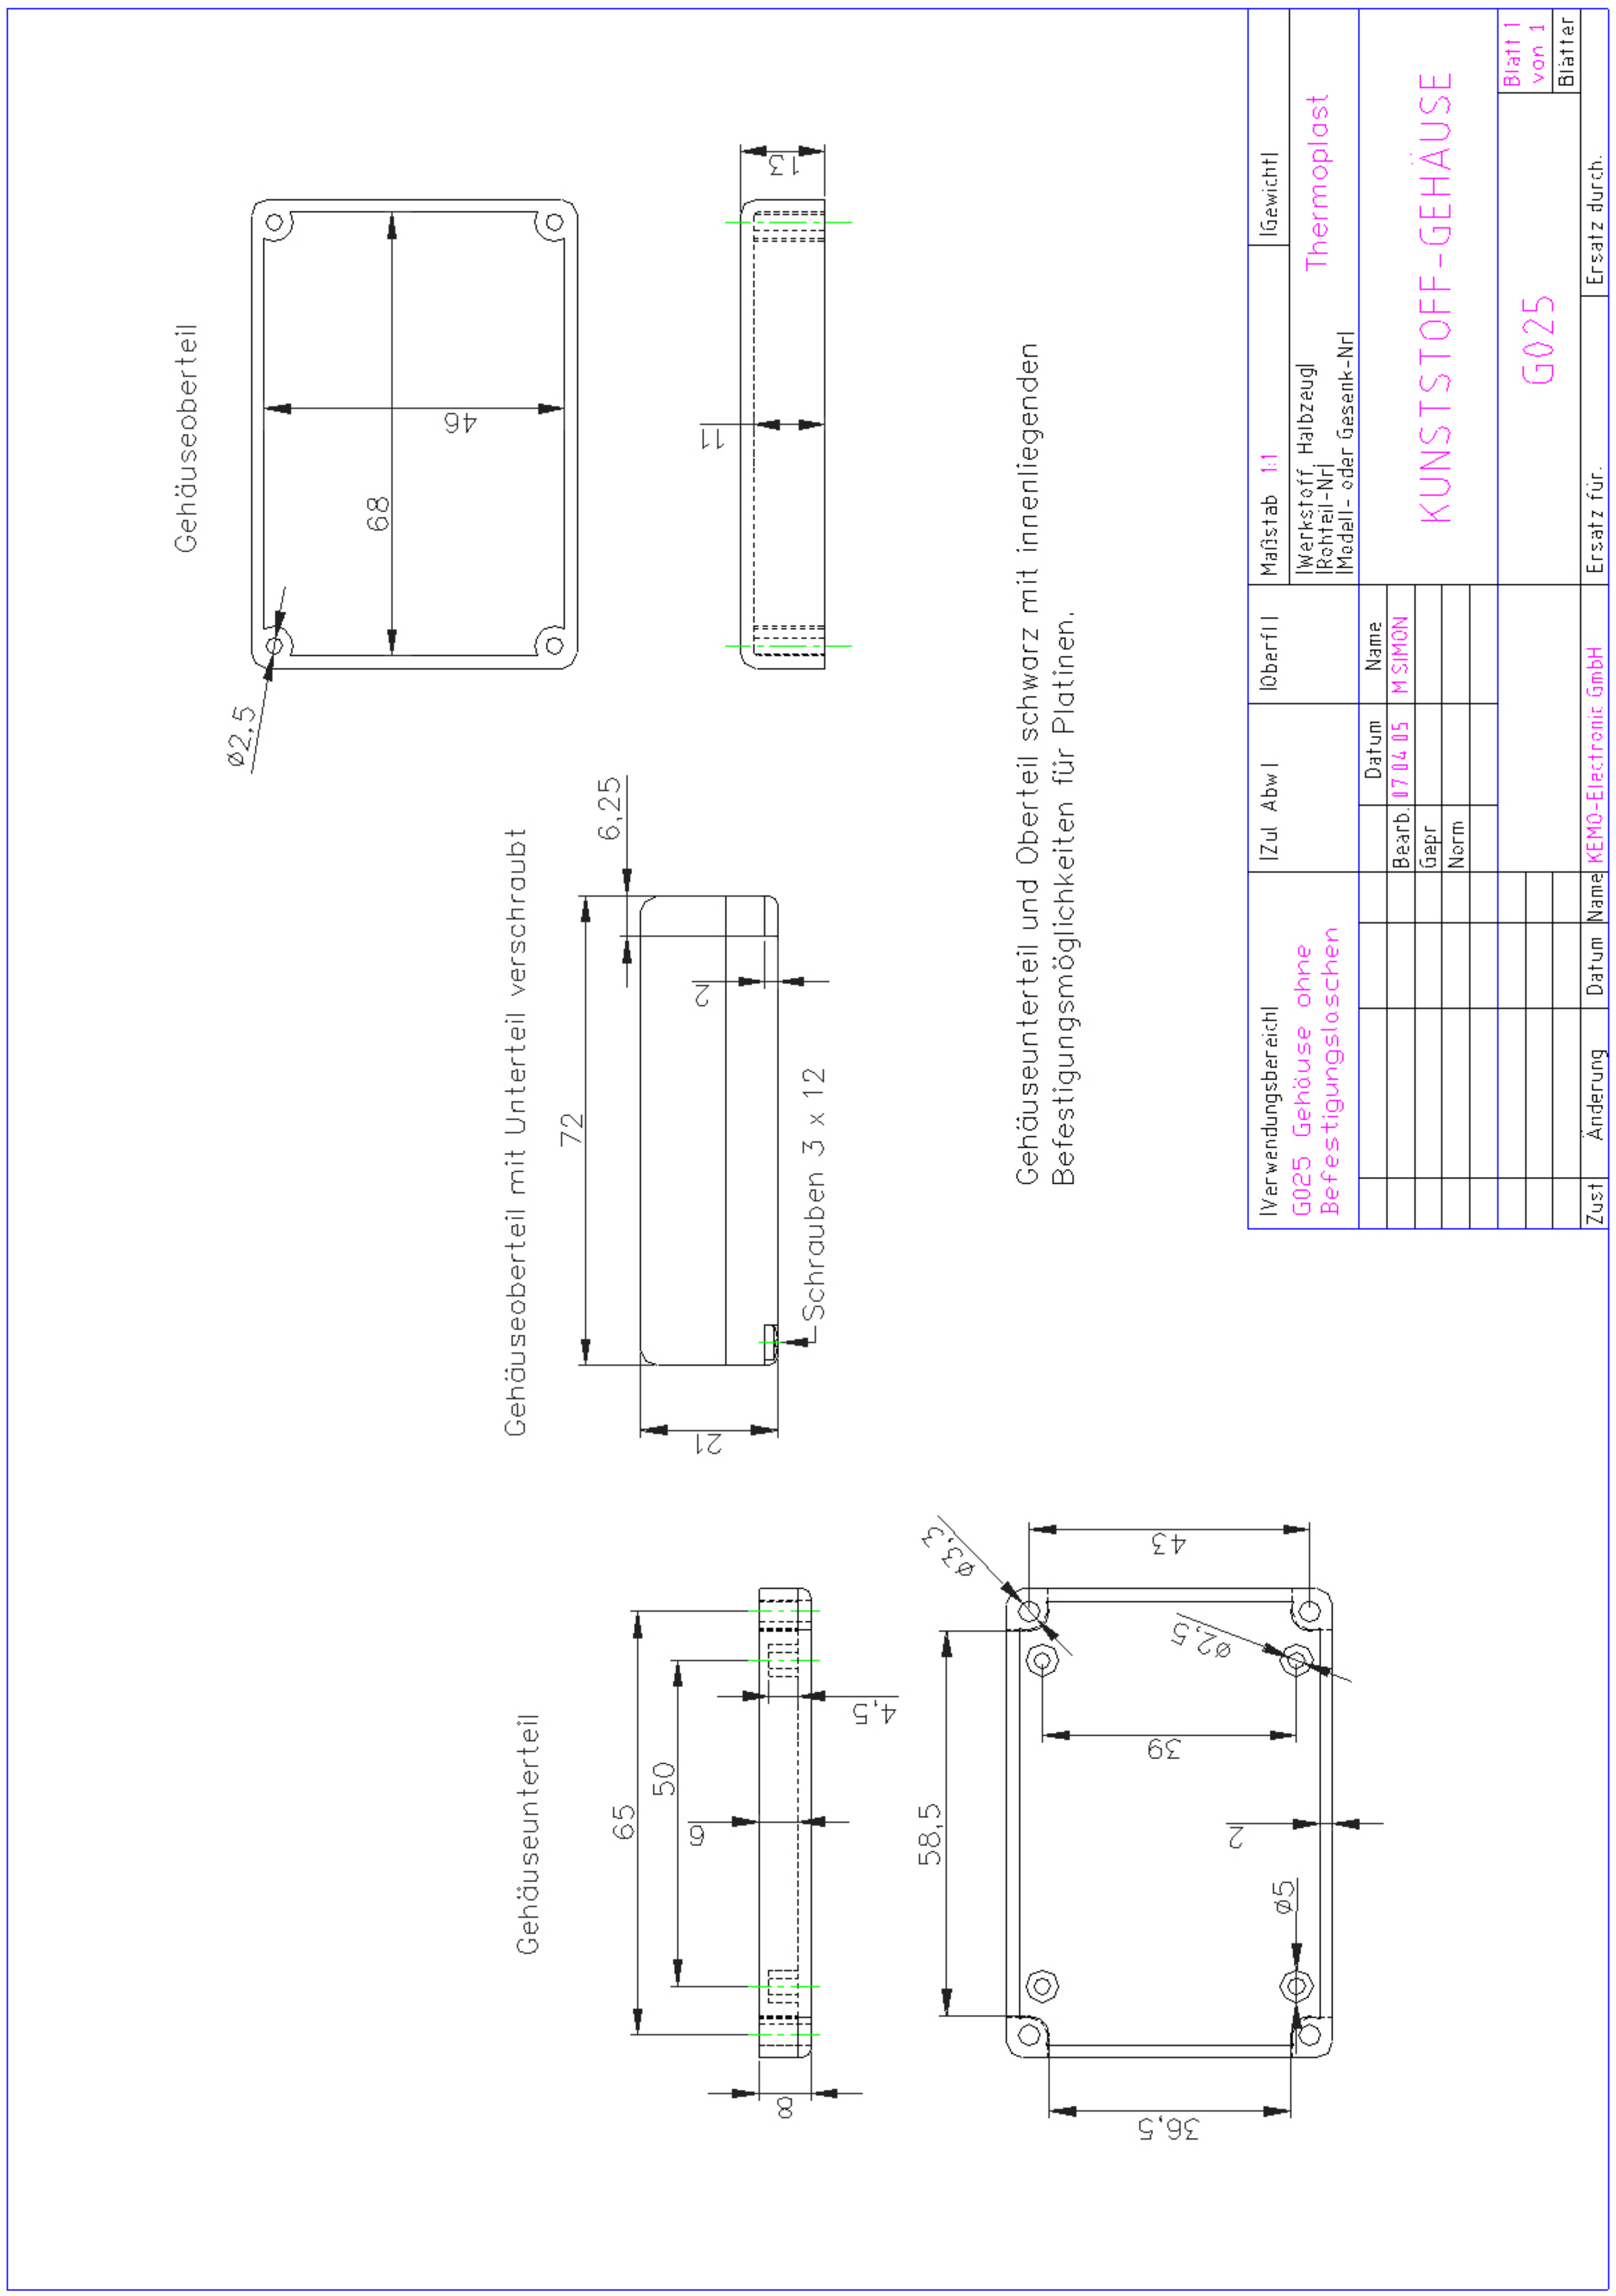
\includegraphics[scale=1]{Gehauseplan.png}


\end{document}
